\documentclass[tikz,border=10pt]{standalone}
\usepackage{amsmath,amssymb,mathtools}
\usetikzlibrary{arrows.meta, decorations.pathreplacing}

% ── Color palette (from cmuts/fig1/overview) ─────────────────────
\definecolor{m0}{HTML}{A44694}     % purple (m=0)
\definecolor{m1}{HTML}{F1A226}     % gold   (m=1)
\definecolor{m2}{HTML}{6DDB5C}     % green  (m=2)
\definecolor{txt}{HTML}{2C2C2C}    % near-black text

% ── Dimensions ────────────────────────────────────────────────────
\def\cs{0.58}   % cell size

\begin{document}
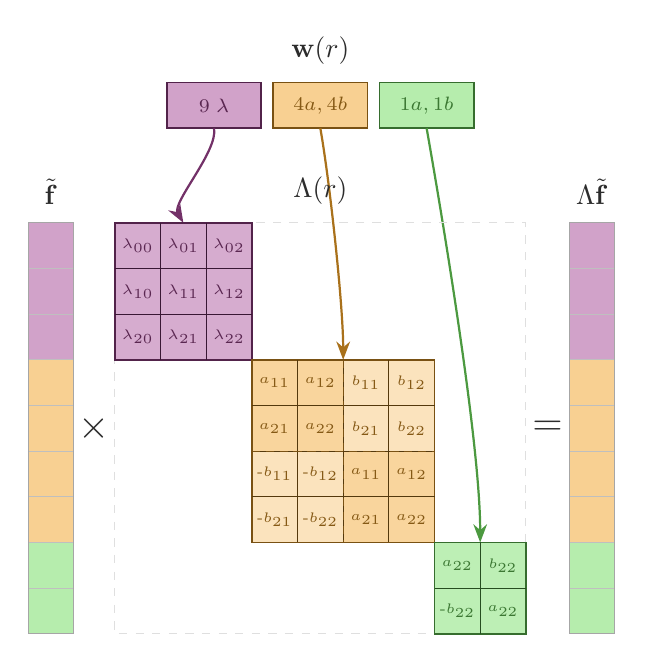
\begin{tikzpicture}[
  >=Stealth,
  every node/.style={font=\small},
  lbl/.style={font=\scriptsize, text=txt},
]

% L = {0,1,2}: p = 1+3+5 = 9
% m-ordered: m=0 (3 entries), m=1 (4 entries), m=2 (2 entries)
\def\N{9}  % matrix dimension
\pgfmathsetmacro{\W}{\N*\cs}
\pgfmathsetmacro{\C}{\W/2}

\def\matX{0.15}
\pgfmathsetmacro{\matR}{\matX+\W}
\def\fvX{-0.95}
\pgfmathsetmacro{\outX}{\matR+0.55}

% Radial weight table dimensions (3 summary blocks)
\pgfmathsetmacro{\matCenter}{\matX+\C}
\def\tblGap{0.15}  % gap between blocks
\def\bW{1.2}       % block width
\pgfmathsetmacro{\tblTotalW}{3*\bW+2*\tblGap}
\pgfmathsetmacro{\tblX}{\matCenter-\tblTotalW/2}
\pgfmathsetmacro{\tblY}{\cs+1.2}

% ── Radial weight table (3 summary blocks) ───────────────────────
\begin{scope}[shift={(\tblX, \tblY)}]
  % m=0 block
  \fill[m0, opacity=0.50] (0, 0) rectangle (\bW, \cs);
  \draw[m0!50!black, semithick] (0, 0) rectangle (\bW, \cs);
  \node[font=\scriptsize, m0!55!black] at ({0.5*\bW}, 0.5*\cs) {$9\;\lambda$};
  % m=1 block
  \pgfmathsetmacro{\bOneX}{\bW+\tblGap}
  \fill[m1, opacity=0.50] (\bOneX, 0) rectangle ({\bOneX+\bW}, \cs);
  \draw[m1!50!black, semithick] (\bOneX, 0) rectangle ({\bOneX+\bW}, \cs);
  \node[font=\scriptsize, m1!55!black] at ({\bOneX+0.5*\bW}, 0.5*\cs) {$4a,4b$};
  % m=2 block
  \pgfmathsetmacro{\bTwoX}{2*\bW+2*\tblGap}
  \fill[m2, opacity=0.50] (\bTwoX, 0) rectangle ({\bTwoX+\bW}, \cs);
  \draw[m2!50!black, semithick] (\bTwoX, 0) rectangle ({\bTwoX+\bW}, \cs);
  \node[font=\scriptsize, m2!55!black] at ({\bTwoX+0.5*\bW}, 0.5*\cs) {$1a,1b$};
  % Label
  \node[font=\normalsize, text=txt, above=3pt] at ({0.5*\tblTotalW}, \cs) {$\mathbf{w}(r)$};
\end{scope}

% Curved arrows from table blocks to corresponding matrix blocks
\draw[->, thick, m0!70!black]
  ({\tblX + 0.5*\bW}, \tblY) to[out=-80, in=120, looseness=0.6]
  ({\matX + 1.5*\cs}, \cs);
\pgfmathsetmacro{\bOneMid}{\tblX+\bW+\tblGap+0.5*\bW}
\draw[->, thick, m1!70!black]
  (\bOneMid, \tblY) to[out=-80, in=90, looseness=0.6]
  ({\matX + 5*\cs}, {-2*\cs});
\pgfmathsetmacro{\bTwoMid}{\tblX+2*\bW+2*\tblGap+0.5*\bW}
\draw[->, thick, m2!70!black]
  (\bTwoMid, \tblY) to[out=-80, in=90, looseness=0.6]
  ({\matX + 8*\cs}, {-6*\cs});

% ── Vertical f̃ (left of matrix) ─────────────────────────────────
\begin{scope}[shift={(\fvX, 0)}]
  % m=0: 3 entries
  \foreach \i in {0,1,2}{\fill[m0, opacity=0.50] (0, {-\i*\cs}) rectangle ++(\cs,\cs);}
  % m=1: 4 entries
  \foreach \i in {0,...,3}{\fill[m1, opacity=0.50] (0, {-(3+\i)*\cs}) rectangle ++(\cs,\cs);}
  % m=2: 2 entries
  \foreach \i in {0,1}{\fill[m2, opacity=0.50] (0, {-(7+\i)*\cs}) rectangle ++(\cs,\cs);}
  \draw[gray!50, thin] (0,\cs) grid[step=\cs] (\cs, {-8*\cs});
  \draw[gray!70] (0,\cs) rectangle (\cs, {-8*\cs});
  \node[font=\normalsize, text=txt, above=3pt] at (0.5*\cs, \cs) {$\tilde{\mathbf{f}}$};
\end{scope}

% × sign (centered between f̃ right edge and matrix left edge)
\node[font=\Large, text=txt] at ({(\fvX+\cs+\matX)/2}, {-3.5*\cs}) {$\times$};

% ── Block-diagonal matrix Λ ──────────────────────────────────────
\begin{scope}[shift={(\matX, 0)}]
  % Dashed ghost outline
  \draw[gray!25, dashed, thin] (0, \cs) rectangle (\W, {-8*\cs});

  % ── m=0 block: 3×3 real matrix (rows 0–2, cols 0–2) ──────────
  % All entries are independent real scalars λ_{ℓ₂ℓ₁}
  \foreach \i in {0,1,2}{
    \foreach \j in {0,1,2}{
      \fill[m0, opacity=0.45] ({\j*\cs}, {-\i*\cs}) rectangle ++(\cs,\cs);
    }
  }
  \draw[m0!50!black, semithick] (0, \cs) rectangle ++({3*\cs}, {-3*\cs});
  % Internal grid
  \foreach \j in {1,2}{\draw[m0!35!black, thin] ({\j*\cs}, \cs) -- ({\j*\cs}, {-2*\cs});}
  \foreach \i in {0,1}{\draw[m0!35!black, thin] (0, {-\i*\cs}) -- ({3*\cs}, {-\i*\cs});}
  % All λ_{ℓ₂ℓ₁} entries (ℓ₁,ℓ₂ ∈ {0,1,2})
  \node[font=\tiny, m0!55!black] at (0.5*\cs, 0.5*\cs) {$\lambda_{00}$};
  \node[font=\tiny, m0!55!black] at (1.5*\cs, 0.5*\cs) {$\lambda_{01}$};
  \node[font=\tiny, m0!55!black] at (2.5*\cs, 0.5*\cs) {$\lambda_{02}$};
  \node[font=\tiny, m0!55!black] at (0.5*\cs, -0.5*\cs) {$\lambda_{10}$};
  \node[font=\tiny, m0!55!black] at (1.5*\cs, -0.5*\cs) {$\lambda_{11}$};
  \node[font=\tiny, m0!55!black] at (2.5*\cs, -0.5*\cs) {$\lambda_{12}$};
  \node[font=\tiny, m0!55!black] at (0.5*\cs, -1.5*\cs) {$\lambda_{20}$};
  \node[font=\tiny, m0!55!black] at (1.5*\cs, -1.5*\cs) {$\lambda_{21}$};
  \node[font=\tiny, m0!55!black] at (2.5*\cs, -1.5*\cs) {$\lambda_{22}$};

  % ── m=1 block: 4×4 with [[A,B],[-B,A]] structure ─────────────
  % rows 3–6, cols 3–6
  % A sub-block (top-left 2×2)
  \foreach \i in {0,1}{
    \foreach \j in {0,1}{
      \fill[m1, opacity=0.45] ({(3+\j)*\cs}, {-(3+\i)*\cs}) rectangle ++(\cs,\cs);
    }
  }
  % B sub-block (top-right 2×2)
  \foreach \i in {0,1}{
    \foreach \j in {0,1}{
      \fill[m1, opacity=0.30] ({(5+\j)*\cs}, {-(3+\i)*\cs}) rectangle ++(\cs,\cs);
    }
  }
  % -B sub-block (bottom-left 2×2)
  \foreach \i in {0,1}{
    \foreach \j in {0,1}{
      \fill[m1, opacity=0.30] ({(3+\j)*\cs}, {-(5+\i)*\cs}) rectangle ++(\cs,\cs);
    }
  }
  % A sub-block (bottom-right 2×2)
  \foreach \i in {0,1}{
    \foreach \j in {0,1}{
      \fill[m1, opacity=0.45] ({(5+\j)*\cs}, {-(5+\i)*\cs}) rectangle ++(\cs,\cs);
    }
  }
  % Outer border
  \draw[m1!50!black, semithick] ({3*\cs}, {-2*\cs}) rectangle ++({4*\cs}, {-4*\cs});
  % Internal grid
  \foreach \j in {4,5,6}{\draw[m1!35!black, thin] ({\j*\cs}, {-2*\cs}) -- ({\j*\cs}, {-6*\cs});}
  \foreach \i in {3,4,5}{\draw[m1!35!black, thin] ({3*\cs}, {-\i*\cs}) -- ({7*\cs}, {-\i*\cs});}
  % Sub-block divider (heavier)
  \draw[m1!50!black, thin, densely dashed]
    ({5*\cs}, {-2*\cs}) -- ({5*\cs}, {-6*\cs});
  \draw[m1!50!black, thin, densely dashed]
    ({3*\cs}, {-4*\cs}) -- ({7*\cs}, {-4*\cs});
  % Individual a_{ℓ₂ℓ₁}, b_{ℓ₂ℓ₁} labels (ℓ₁,ℓ₂ ∈ {1,2})
  % A sub-block (top-left)
  \node[font=\tiny, m1!55!black] at (3.5*\cs, -2.5*\cs) {$a_{11}$};
  \node[font=\tiny, m1!55!black] at (4.5*\cs, -2.5*\cs) {$a_{12}$};
  \node[font=\tiny, m1!55!black] at (3.5*\cs, -3.5*\cs) {$a_{21}$};
  \node[font=\tiny, m1!55!black] at (4.5*\cs, -3.5*\cs) {$a_{22}$};
  % B sub-block (top-right)
  \node[font=\tiny, m1!55!black] at (5.5*\cs, -2.5*\cs) {$b_{11}$};
  \node[font=\tiny, m1!55!black] at (6.5*\cs, -2.5*\cs) {$b_{12}$};
  \node[font=\tiny, m1!55!black] at (5.5*\cs, -3.5*\cs) {$b_{21}$};
  \node[font=\tiny, m1!55!black] at (6.5*\cs, -3.5*\cs) {$b_{22}$};
  % -B sub-block (bottom-left)
  \node[font=\tiny, m1!55!black] at (3.5*\cs, -4.5*\cs) {$\text{-}b_{11}$};
  \node[font=\tiny, m1!55!black] at (4.5*\cs, -4.5*\cs) {$\text{-}b_{12}$};
  \node[font=\tiny, m1!55!black] at (3.5*\cs, -5.5*\cs) {$\text{-}b_{21}$};
  \node[font=\tiny, m1!55!black] at (4.5*\cs, -5.5*\cs) {$\text{-}b_{22}$};
  % A sub-block (bottom-right)
  \node[font=\tiny, m1!55!black] at (5.5*\cs, -4.5*\cs) {$a_{11}$};
  \node[font=\tiny, m1!55!black] at (6.5*\cs, -4.5*\cs) {$a_{12}$};
  \node[font=\tiny, m1!55!black] at (5.5*\cs, -5.5*\cs) {$a_{21}$};
  \node[font=\tiny, m1!55!black] at (6.5*\cs, -5.5*\cs) {$a_{22}$};

  % ── m=2 block: 2×2 rotation-scaling (rows 7–8, cols 7–8) ─────
  \fill[m2, opacity=0.45] ({7*\cs}, {-7*\cs}) rectangle ++(\cs,\cs);
  \node[font=\tiny, m2!55!black] at (7.5*\cs, -6.5*\cs) {$a_{22}$};
  \fill[m2, opacity=0.45] ({8*\cs}, {-7*\cs}) rectangle ++(\cs,\cs);
  \node[font=\tiny, m2!55!black] at (8.5*\cs, -6.5*\cs) {$b_{22}$};
  \fill[m2, opacity=0.45] ({7*\cs}, {-8*\cs}) rectangle ++(\cs,\cs);
  \node[font=\tiny, m2!55!black] at (7.5*\cs, -7.5*\cs) {$\text{-}b_{22}$};
  \fill[m2, opacity=0.45] ({8*\cs}, {-8*\cs}) rectangle ++(\cs,\cs);
  \node[font=\tiny, m2!55!black] at (8.5*\cs, -7.5*\cs) {$a_{22}$};
  \draw[m2!50!black, semithick] ({7*\cs}, {-6*\cs}) rectangle ++({2*\cs}, {-2*\cs});
  \draw[m2!35!black, thin] ({8*\cs}, {-6*\cs}) -- ({8*\cs}, {-8*\cs});
  \draw[m2!35!black, thin] ({7*\cs}, {-7*\cs}) -- ({9*\cs}, {-7*\cs});

  % Label
  \node[font=\normalsize, text=txt, above=3pt] at (\C, \cs) {$\Lambda(r)$};

\end{scope}

% = sign (centered between matrix right edge and Λf̃ left edge)
\node[font=\Large, text=txt] at ({(\matR+\outX)/2}, {-3.5*\cs}) {$=$};

% ── Vertical Λf̃ (right of matrix) ───────────────────────────────
\begin{scope}[shift={(\outX, 0)}]
  \foreach \i in {0,1,2}{\fill[m0, opacity=0.50] (0, {-\i*\cs}) rectangle ++(\cs,\cs);}
  \foreach \i in {0,...,3}{\fill[m1, opacity=0.50] (0, {-(3+\i)*\cs}) rectangle ++(\cs,\cs);}
  \foreach \i in {0,1}{\fill[m2, opacity=0.50] (0, {-(7+\i)*\cs}) rectangle ++(\cs,\cs);}
  \draw[gray!50, thin] (0,\cs) grid[step=\cs] (\cs, {-8*\cs});
  \draw[gray!70] (0,\cs) rectangle (\cs, {-8*\cs});
  \node[font=\normalsize, text=txt, above=3pt] at (0.5*\cs, \cs) {$\Lambda\tilde{\mathbf{f}}$};
\end{scope}

\end{tikzpicture}
\end{document}
